% https://www.overleaf.com/learn/latex/Beamer#Introduction
% https://en.wikibooks.org/wiki/LaTeX/Presentations#The_Beamer_package
\documentclass{beamer}
\usepackage[utf8]{inputenc}
% http://texblog.net/latex-archive/latex-general/beamer-warnings/
\usepackage{lmodern}
% https://hartwork.org/beamer-theme-matrix/
% \usecolortheme{dove}

% https://tex.stackexchange.com/a/356169
\usepackage[style=ieee,backend=bibtex]{biblatex}
\addbibresource{bibliography.bib}

\beamertemplatenavigationsymbolsempty
% https://tex.stackexchange.com/a/74251
\setbeamerfont{page number in head/foot}{size=\small}
\setbeamertemplate{footline}[frame number]
\setbeamerfont{footnote}{size=\tiny}
 
\author{Russel Shawn Dsouza}
% https://tex.stackexchange.com/a/61053
\institute
{
  
\includegraphics[scale=0.25]{images/logo}\\
  Electronics and Communications Engg.\\
  National Institute of Technology Karnataka\\
  Surathkal, India - 575025
}
\date{October 9, 2019}

\title[Neural TTS]{Neural Text-to-Speech}
% \subtitle{A short story}
 
\begin{document}

  % https://stackoverflow.com/a/54916411
  \begingroup
    \setbeamertemplate{footline}{}
    \frame{\titlepage}
  \endgroup

  \addtocounter{framenumber}{-1}

  % https://tex.stackexchange.com/a/198102
  % \begin{frame}{Overview}
  %   \tableofcontents
  % \end{frame}

  \begin{frame}
    \frametitle{Speech synthesis}
      Artificial production of human speech
      \begin{figure}
        \centering
        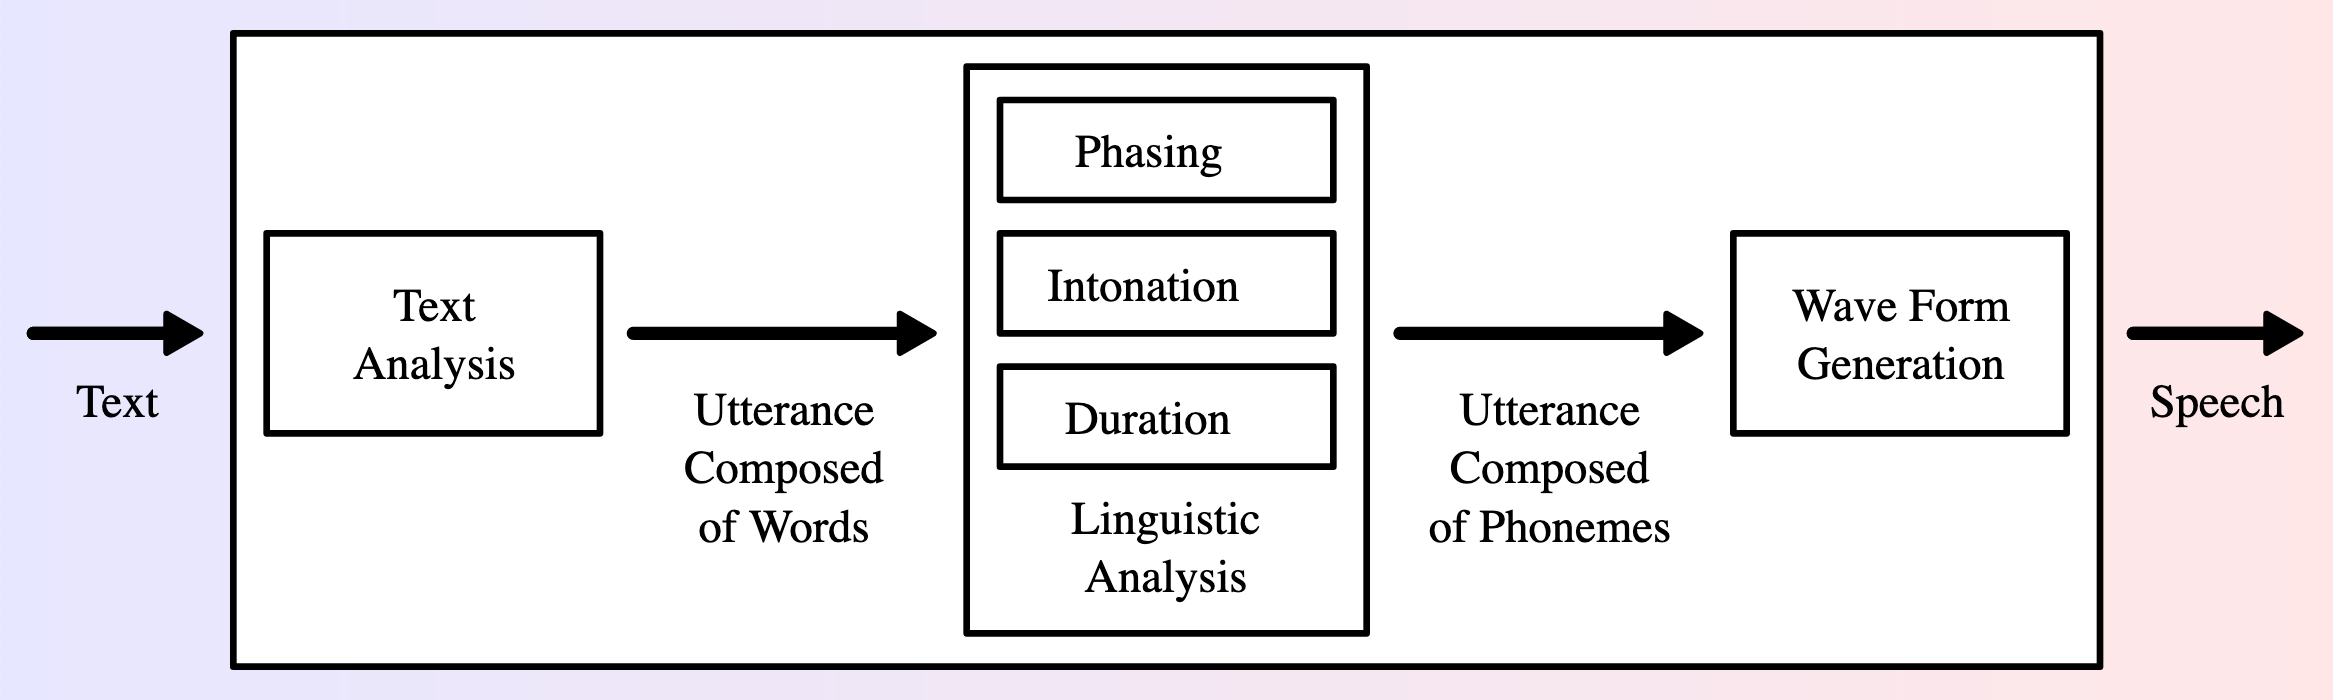
\includegraphics[width=\textwidth]{images/TTS_System_screenshot}
        \caption{A typical text-to-speech system\footfullcite{wiki_tts}}
      \end{figure}
  \end{frame}

  \begin{frame}
    \frametitle{History of speech synthesis}
    % TODO: Add images for each type
      \begin{columns}
        \column{0.33\textwidth}
          \textbf{Concatenative}\\
          \begin{itemize}
            \item Extract samples from large database of human speech
          \end{itemize}

        \column{0.33\textwidth}
          \textbf{Parametric}\\
          \begin{itemize}
            \item Simulate human voice using a parametric function
          \end{itemize}

        \column{0.33\textwidth}
          \textbf{Neural}\\
          \begin{itemize}
            \item Artificially generate human voice using neural networks
          \end{itemize}
      \end{columns}
  \end{frame}

  \begin{frame}
    \frametitle{Approaches in Neural text-to-speech}
      \begin{itemize}
          \item LSTM
          \item WaveNet
          \item WaveNet based
      \end{itemize}
  \end{frame}

  \begin{frame}
    \frametitle{WaveNet}
      A deep neural network for generating raw audiowaveforms.

      \begin{itemize}
        \item Probabilistic 
        \item Autoregressive
        \item Beats all previously known methods
      \end{itemize}
      \begin{figure}
        \centering
        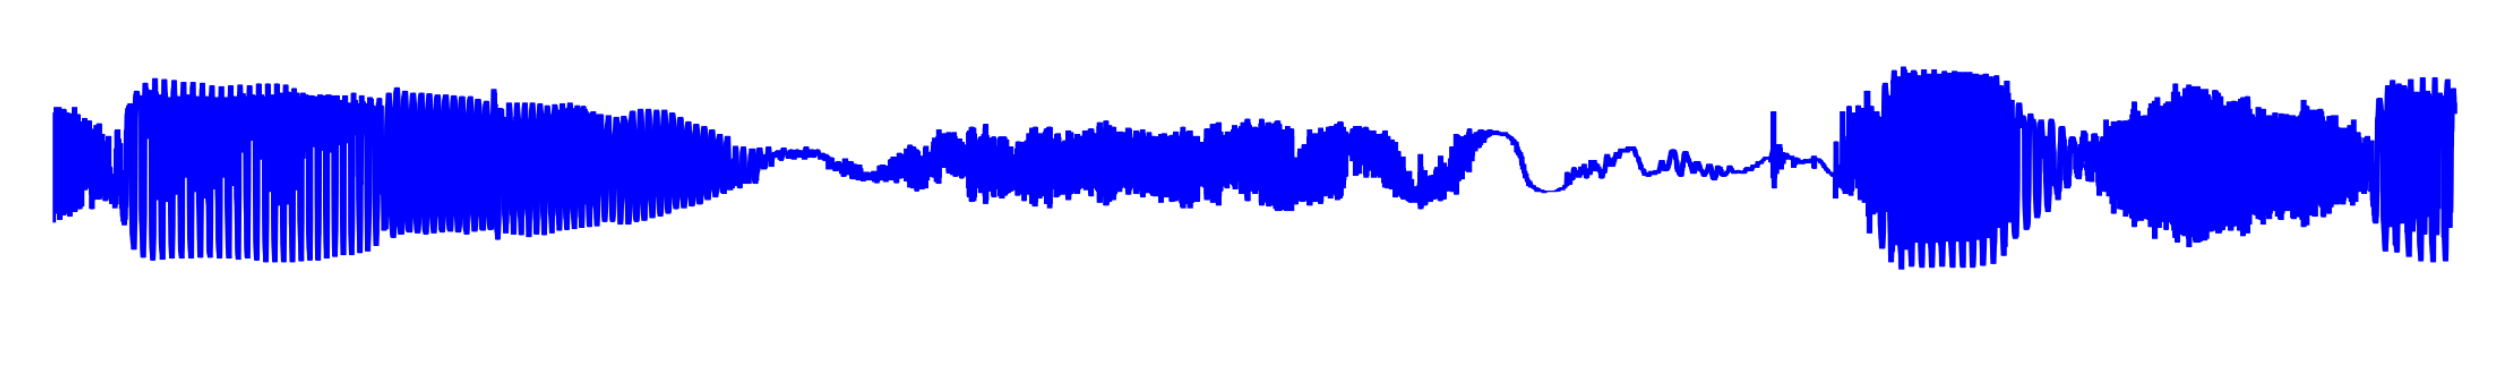
\includegraphics[width=\textwidth]{images/second_of_speech.png}
        \caption{Time domain representation of 1 second of generated speech}
      \end{figure}
  \end{frame}

  \begin{frame}
    \frametitle{WaveNet: Architecture}
      \begin{itemize}
        \item Dilated convolution
        \item $\mu$ law companding
        \item Gated activation
        \item Residual and skip connection
        \item Conditional wavenets
      \end{itemize}
  \end{frame}

  \begin{frame}
    \frametitle{1. Dilated Convolution}
    \begin{figure}
      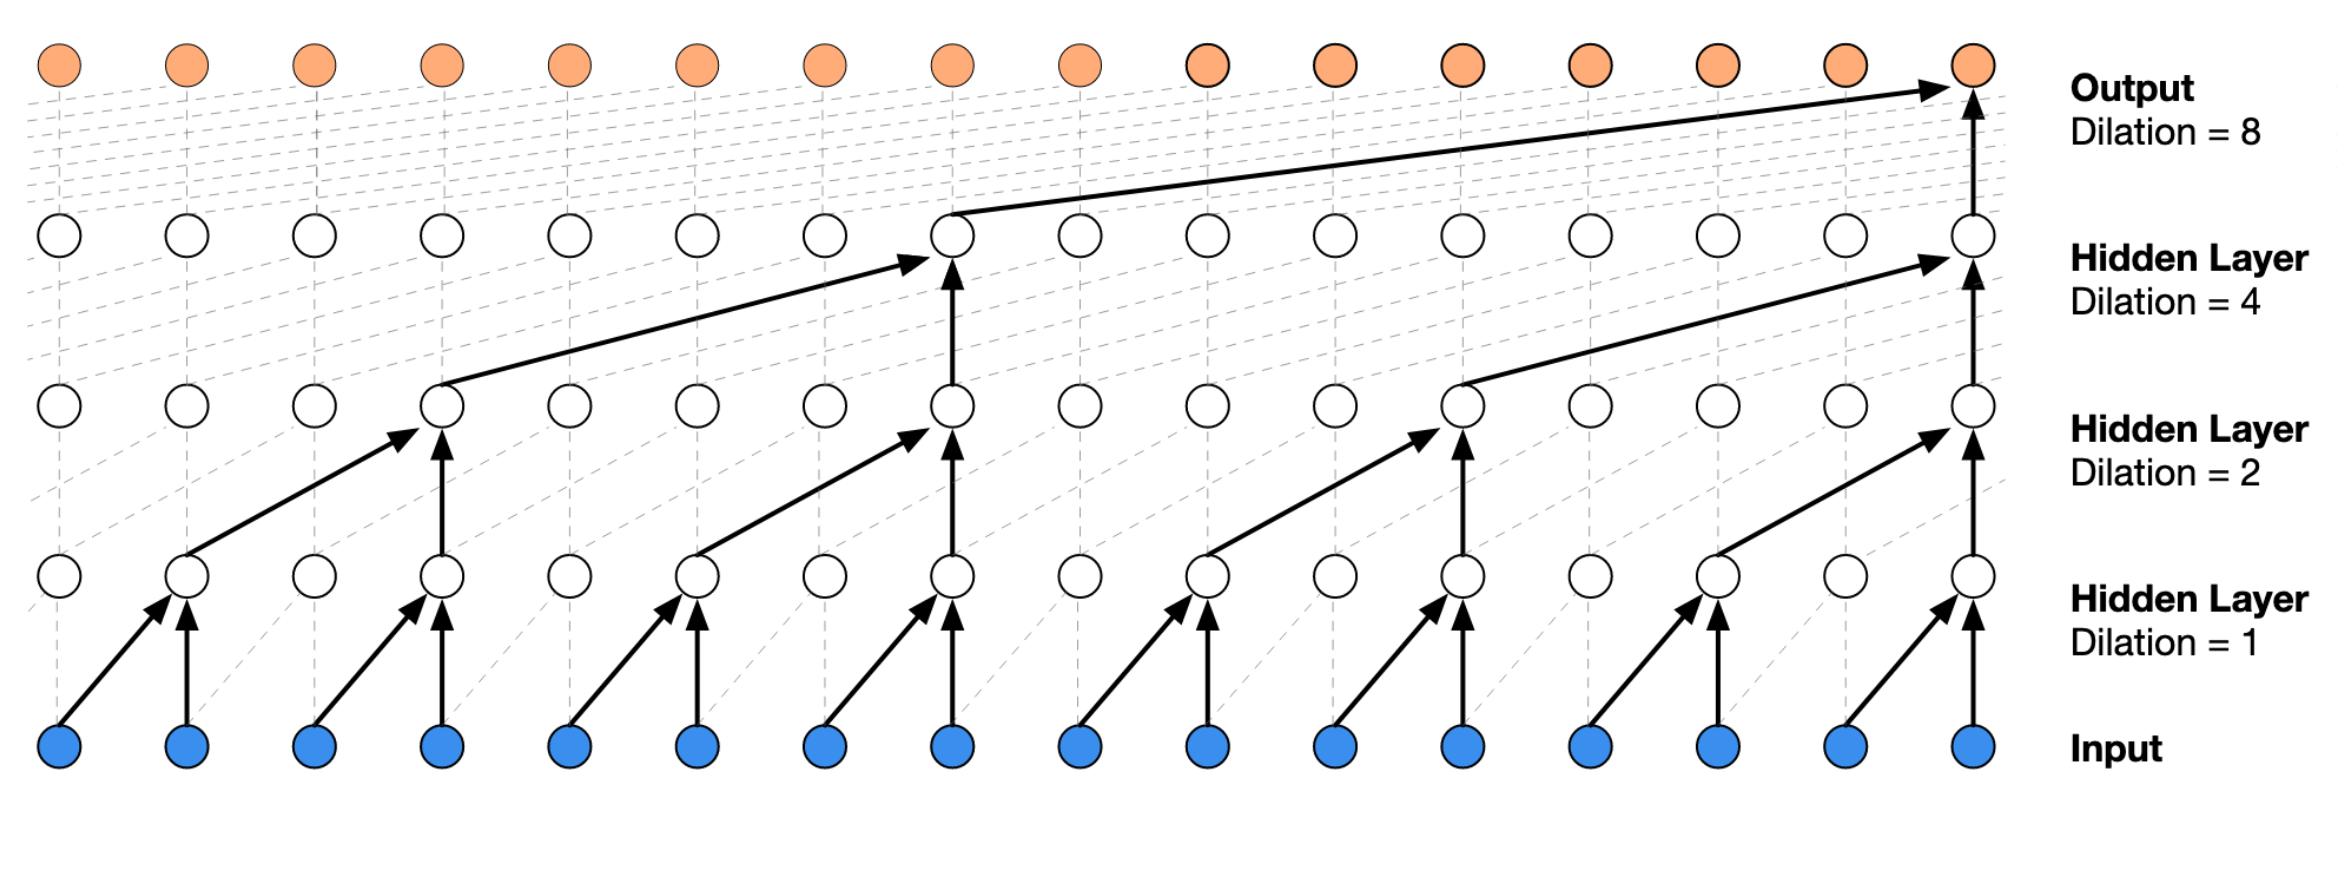
\includegraphics[scale=0.22]{images/wavenet_arch_dilated_conv.png}
      \caption{Stack of dilated causal convolution layers\footfullcite{oord_wavenet:_2016}}
    \end{figure}
  \end{frame}

  \begin{frame}
    \frametitle{2. $\mu$-law companding}
    \centering
    % TODO: Explain equation
    \begin{equation*}
      f(x_t) = \text{sign}(x_t)\frac{\ln(1 + \mu|x_t|)}{\ln(1 + \mu)}
    \end{equation*}
    where, $x_t$ is the time domain speech signal
  \end{frame}

  \begin{frame}
    \frametitle{3. Gated activation}
    \centering
    % TODO: Explain equation
    \begin{equation*}
      \mathbf{z} = \tanh(W_{f, k}*\mathbf{x}) \circledast \sigma (W_{g, k}*\mathbf{x})
    \end{equation*}
    \begin{flushleft}
    $* \rightarrow$ convolution,\\
    $\circledast \rightarrow$ element-wise multiplication,\\
    $\sigma\text{(.)} \rightarrow$ sigmoid function,\\
    $k \rightarrow$ layer index,\\
    $f \rightarrow$ filter,\\
    $g \rightarrow$ gate,\\
    $W \rightarrow$ learnable convolution filter\footfullcite{oord_conditional_2016}
    \end{flushleft}
  \end{frame}

  \begin{frame}
    \frametitle{4. Residual and skip connections}
    \begin{figure}[ht]
      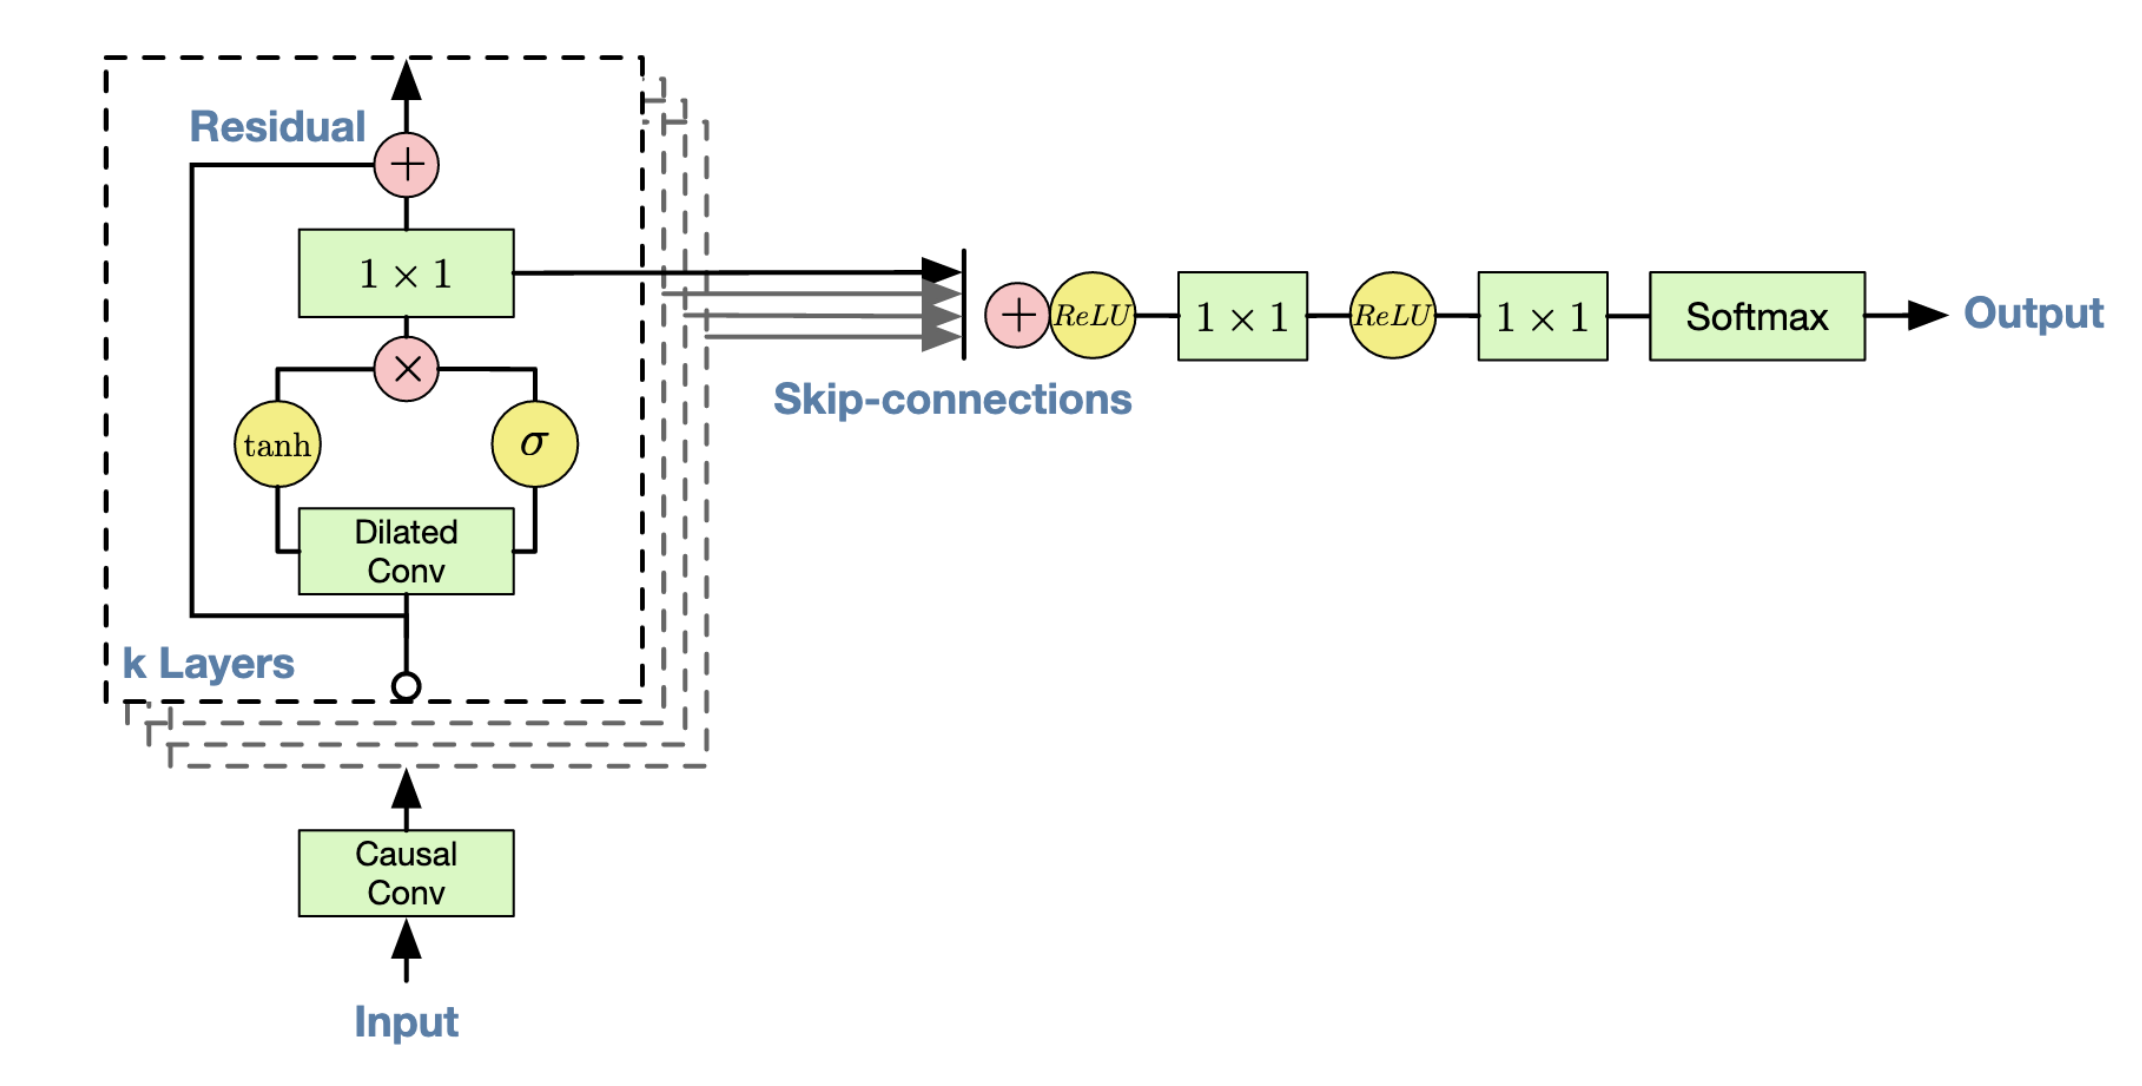
\includegraphics[width=\textwidth]{images/wavenet_arch_residual.png}
      \caption{Overview of residual block and entire architecture \footfullcite{oord_wavenet:_2016}}
    \end{figure}
  \end{frame}

  \begin{frame}
    \frametitle{5. Conditional WaveNets}
    % TODO: Explain equation
    \begin{equation*}
      p(\mathbf{x} | \mathbf{h}) = \prod_{t=1}^{T}p(x_t | x_1, \ldots, x_{t-1}, \mathbf{h}) 
    \end{equation*}
  \end{frame}

  \begin{frame}
    \frametitle{WaveNet: Pros and Cons}
    \begin{columns}
      \column{0.5\textwidth}
        \textbf{Pros}
        \begin{itemize}
          \item Fast training
        \end{itemize}
      \column{0.5\textwidth}
        \textbf{Cons}
        \begin{itemize}
          \item Slow inference
        \end{itemize}
    \end{columns}
  \end{frame}

  \begin{frame}
    \frametitle{Tacotron 2: Architecture}
    \begin{figure}
      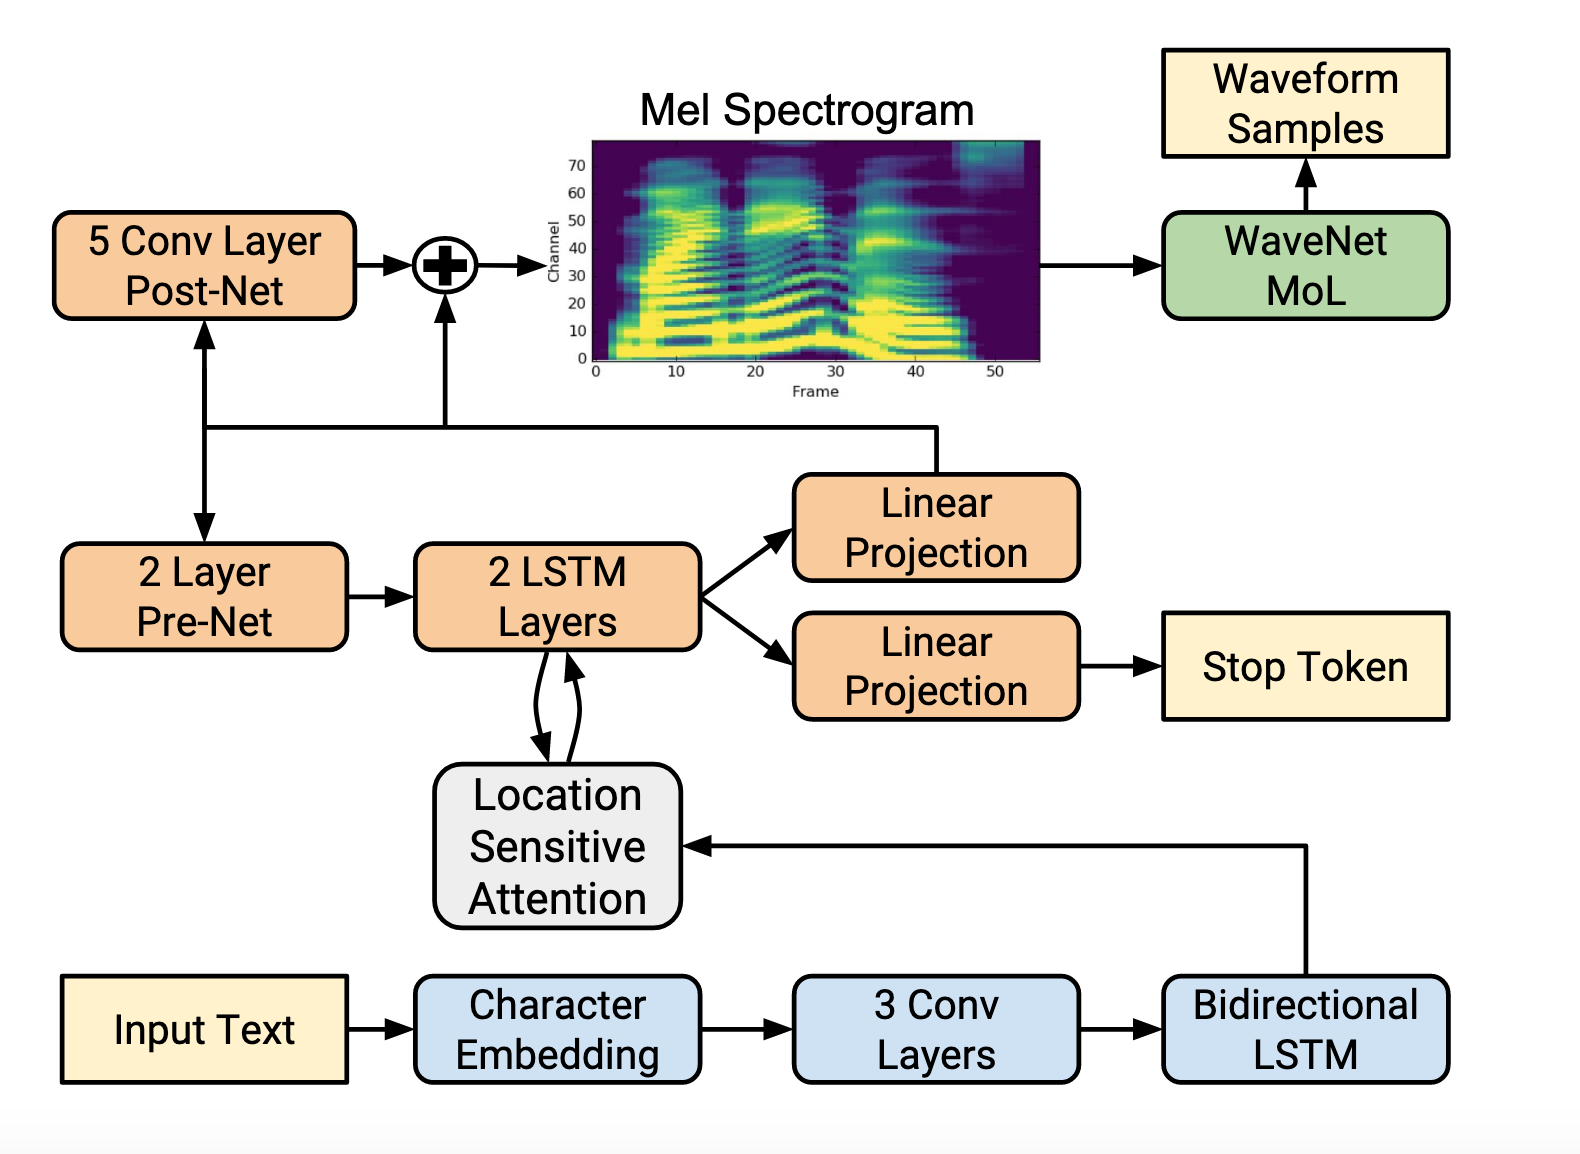
\includegraphics[scale=0.25]{images/tacotron_arch.png}
      \caption{Block diagram of Tacotron 2 system architecture\footfullcite{shen_natural_2017}}
    \end{figure}
  \end{frame}

  \begin{frame}
    \frametitle{Mel spectrogram}
      \begin{itemize}
        \item Related to the short-time Fourier transform (STFT) magnitude 
        \item Obtained by applying a nonlinear transform to the frequency axis of the STFT
        \item Emphasizes details in lower frequencies
        \item De-emphasizes high frequency details
      \end{itemize}
      Features derived from the mel scale have been used as an underlying representation for speech recognition for many decades. \footfullcite{davis1980comparison}
  \end{frame}

  \begin{frame}
    \frametitle{Tacotron 2: Training}
    \begin{columns}
      \column{0.5\textwidth}
        \textbf{Feature detection}
        \begin{itemize}
          \item Maximum likelihood training procedure
          \item Batch size = 64 on a single GPU
          \item Adam optimizer w/ $\beta_1=0.9$, $\beta_2=0.999$, $\epsilon=10^{-6}$
          \item LR = $10^{-3}$, exponentially decaying to $10^{-5}$
          \item Warmup training till 50,000 iterations
          \item L2 regularization with weight $10^{-6}$
        \end{itemize}
      \column{0.5\textwidth}
        \textbf{WaveNet}
        \begin{itemize}
          \item Batch size = 128 on 32 GPUs
          \item Adam optimizer w/ $\beta_1=0.9$, $\beta_2=0.999$, $\epsilon=10^{-8}$
          \item Fixed LR = $10^{-4}$
          \item Exponentially-weighted moving average of the network parameters over update steps with a decay of 0.9999
          \item Scaling by 127.5
          \item US English dataset
        \end{itemize}
    \end{columns}
  \end{frame}

  \begin{frame}
    \frametitle{Tactron 2: Evaluation}
    \begin{itemize}
      \item 100 random examples from test set sent to Mechanical Turk
      \item Each sample is rated by atleast 8 raters
      \item Scores on a scale of 1 to 5 with 0.5 increments
    \end{itemize}
  \end{frame}

  \begin{frame}
    \frametitle{Tacotron 2: Reported results}
    \begin{figure}
      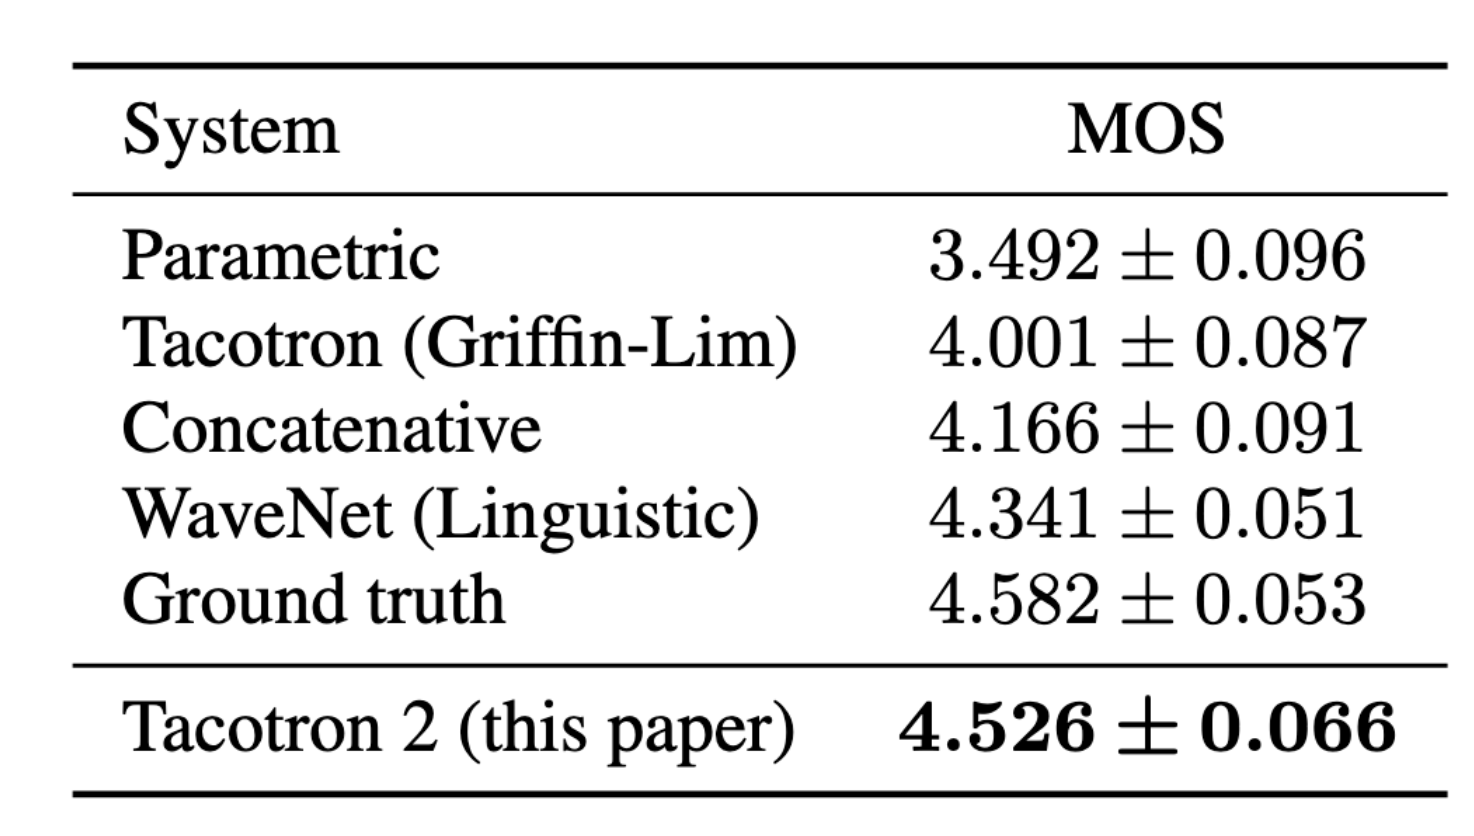
\includegraphics[scale=0.3]{images/tacotron_results.png}
      \caption{Mean Opinion Score (MOS) evaluations}\footfullcite{shen_natural_2017}
    \end{figure}
  \end{frame}

  \begin{frame}
    \frametitle{Summary}
  \end{frame}
  
\end{document}
